\documentclass{article}
\usepackage{tikz}
\usetikzlibrary{calc,positioning,shadows.blur,matrix,decorations.markings,decorations.pathreplacing}
\usepackage{etoolbox}

\definecolor{colone}{RGB}{209,220,204}
\definecolor{coltwo}{RGB}{204,222,210}
\definecolor{colthree}{RGB}{207,233,232}
\definecolor{colfour}{RGB}{248,243,214}
\definecolor{colfive}{RGB}{245,238,197}
\definecolor{colsix}{RGB}{243,235,179}
\definecolor{colseven}{RGB}{241,231,163}


\tikzset{%
        brace/.style = { decorate, decoration={brace, amplitude=5pt} },
       mbrace/.style = { decorate, decoration={brace, amplitude=5pt, mirror} },
        label/.style = { black, midway, scale=0.5, align=center },
     toplabel/.style = { label, above=.5em, anchor=south },
    leftlabel/.style = { label,rotate=-90,left=.5em,anchor=north },
  bottomlabel/.style = { label, below=.5em, anchor=north },
        force/.style = { rotate=-90,scale=0.4 },
        round/.style = { rounded corners=2mm },
       legend/.style = { right,scale=0.4 },
        nosep/.style = { inner sep=0pt },
   generation/.style = { anchor=base }
}



\begin{document}

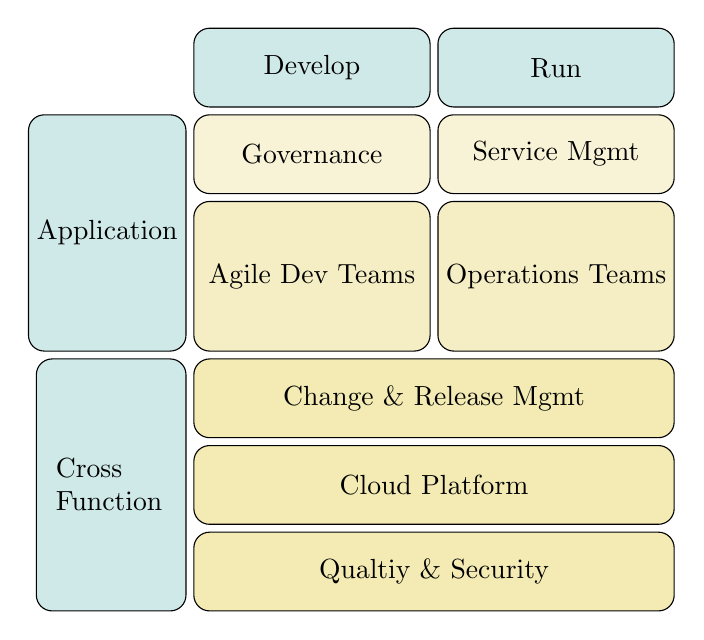
\begin{tikzpicture}

  \draw [round, fill=colthree] (1,0) rectangle (4,-1) node[pos=.5]{Develop};
  \draw[round, fill=colthree] (4.1,0) rectangle (7.1,-1) node[pos=.5]{Run};
  \draw[round, fill=colthree]  (-1.1,-1.1) rectangle (.9,-4.1) node[pos=.5]{Application};
  \draw[round, fill=colthree]  (-1,-4.2) rectangle (.9,-7.4) node[pos=.5, text width=4em]{{Cross\\ Function}};
  \draw[round, fill=colfour]  (1,-1.1) rectangle (4, -2.1) node[pos=.5]{Governance};
  \draw[round, fill=colfour]  (4.1,-1.1) rectangle (7.1,-2.1) node[pos=.5] {Service Mgmt};
  \draw[round, fill=colfive]  (1,-2.2) rectangle (4, -4.1) node[pos=.5]{Agile Dev Teams};
  \draw[round, fill=colfive]  (4.1,-2.2) rectangle (7.1,-4.1) node[pos=.5]{Operations Teams};
  \draw[round, fill=colsix]   (1,-4.2) rectangle (7.1,-5.2) node[pos=.5]{Change \& Release Mgmt};
  \draw[round, fill=colsix]   (1,-5.3) rectangle (7.1,-6.3) node[pos=.5]{Cloud Platform};
  \draw[round, fill=colsix]   (1,-6.4) rectangle (7.1,-7.4) node[pos=.5]{Qualtiy \& Security};

\end{tikzpicture}
\end{document}
